\chapter{Quá trình quyết định Markov - MDP}
\label{ch:03}
Quá trình quyết định Markov (MDP) cung cấp một nền tảng toán học cho việc mô hình hóa ra quyết định trong các tình huống mà kết quả có yếu tố ngẫu nhiên và/hoặc phụ thuộc vào sự điều khiển của một người ra quyết định. MDP được sử dụng rất nhiều các lĩnh vực khác nhau, bao gồm robot, điều khiển tự động, kinh tế, chế tạo,~\dots Trong phần này, chúng ta sẽ trình bày về quá trình quyết định Markov trong đó tập trung vào các khái niệm của quá trình Markov có số bước vô hạn và hữu hạn. Kiến thức trong phần này được tổng hợp từ các tài liệu~\cite{Belman1957},~\cite{Sutton1999} và~\cite{Puterman1994}.
\section{Khái niệm}
Một quá trình quyết định Markov (\textit{Markov Decision Process}) là một quá trình phần thưởng Markov (\textit{Markov Reward Process}) với các quyết định. Trong đó, tất cả các trạng thái đều thỏa mãn tính Markov. Cụ thể:
\begin{dn}\rm
(Quá trình quyết định Markov) Một quá trình quyết định Markov là một bộ năm thành phần $(S,A,P(.|.,.),R(.,.),\gamma)$, trong đó:
\begin{itemize}
 \item $S$ là một tập hữu hạn các trạng thái, kí hiệu $S_t$ là trạng thái tại thời điểm $t$; 
 \item $A$ là một tập hữu hạn các hành động, kí hiệu $A_t$ là hành động tại thời điểm $t (A(s)$ là tập hữu hạn các hành động có sẵn từ trạng thái $s$ với $s\in S)$;
 \item $Pr_{a}(s,s')=Pr(S_{t+1}=s'|S_t=s,A_t=a)$ là xác suất mà hành động $a$ tại trạng thái $s$ ở thời điểm $t$ chuyển sang trạng thái $s'$ tại thời điểm $t+1$. Xác suất này thỏa mãn tính Markov, nghĩa là:
 \begin{align*}
 Pr(S_{t+1}=j|S_0,A_0,...,S_t,A_t)=Pr(S_{t+1}=j|S_t,A_t);
 \end{align*}
 \item $R_a(s,s')$ là phần thưởng nhận được khi chọn hành động $s$ để chuyển trạng thái từ $s$ sang $s'$;
 \item $\gamma \in [0,1]$ là hệ số suy giảm, đại diện cho sự khác biệt giữa các phần thưởng trong tương lai và phần thưởng hiện tại.
\end{itemize}
\begin{figure}[ht]
    \centering
    \begin{center}
    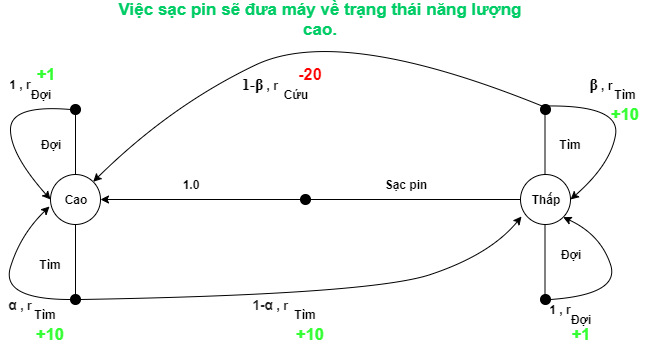
\includegraphics[scale=0.8]{ViduDnMDP.png}
    \end{center}    
    \caption{Quá trình chuyển trạng thái của sinh viên.}
    \label{fig:ViduDnMDP}
\end{figure}
\end{dn}
\begin{vd} \rm: Máy bán hàng tự động
\begin{itemize}
\item Trạng thái: cấu hình các khe.
\item Hành động: thời gian dừng lại.
\item Mục tiêu: kiếm được nhiều tiền.
\item Bài toán: tìm $\pi:S\to A$ sao cho $R$ lớn nhất.
\end{itemize}
\end{vd}
\begin{dn}\rm
(Chiến lược quyết định). Một\textit{ chiến lược }$\pi$ là một phân phối các hành động tại mỗi trạng thái:
\begin{align*}
\pi (a|s)=Pr[A_t=a|S_t=s].
\end{align*}
Một số kiểu chiến lược như sau:
\begin{itemize}
\item $\pi=(\pi^0,...,\pi^{T-1})$ được gọi là \textit{một chiến lược Markov} nếu tại mỗi thời điểm $n$, quyết định $\pi^n$ không phụ thuộc vào quá khứ $h_{n-1}$.\\
 Ví dụ: \begin{align*}
 \pi_{h_{n-1,i_n}}^{n}(a)=\pi_{h'_{n-1,i_n}}^{n}(a),~ a \in A(i_n), ~i_n \in S ~\forall ~h_{n-1},~h'_{n-1}.
 \end{align*}
 \item $\pi$ được gọi là một chiến lược dừng nếu mọi quy tắc quyết định đều bằng nhau :
 \begin{align*}
 \pi^n=\pi^0~~\text{với}~~n=0,1,...,T-1.
 \end{align*}
\end{itemize}
Trong quá trình quyết định Markov, mỗi chiến lược xác định đầy đủ hành động của một tác nhân. Ngoài ra, các chiến lược này chỉ phụ thuộc vào trạng thái của xích Markov tại thời điểm hiện tại (không phụ thuộc vào quá khứ).
\end{dn}
\section{Bài toán quyết định Markov}
\subsection{Phát biểu bài toán}
Bài toán quyết định Markov là bài toán học từ các tác động để đạt được mục đích. Người học và người ra quyết định được gọi là tác tử. Tất cả những gì mà chúng tương tác với, bao gồm mọi thứ bên ngoài tác tử được gọi là môi trường. Các tác động thực hiện một cách liên tục, tác tử lựa chọn hành động, môi trường đáp ứng lại các hành động đó và chuyển từ trạng thái hiện thời sang trạng thái mới. Môi trường cũng đem lại các mục tiêu, các giá trị hằng số mà tác tử cố gắng cực đại hóa qua thời gian. Một đặc tả hoàn thiện về môi trường được coi là một "nhiệm vụ", một thực thể của bài toán quyết định Markov.\\
Tóm lại, bài toán quyết định Markov liên quan đến lớp bài toán trong đó một tác tử rút ra kết luận trong khi phân tích một chuỗi các hành động của nó cùng với tín hiệu vô hướng được đưa ra bởi môi trường.\\
Trong khái niệm chung này, có thể thấy hai đặc tính quan trọng:
\begin{itemize}
\item Tác tử tương tác với môi trường và cặp "tác tử + môi trường" tạo thành một hệ thống động.
\item Tín hiệu tăng cường, được nhận biết dựa vào mục tiêu, cho phép tác tử thay đổi hành vi của nó.
\end{itemize}
Lược đồ tương tác tác tử-môi trường như sau:\\
\newpage
\begin{figure}[ht]
    \centering
    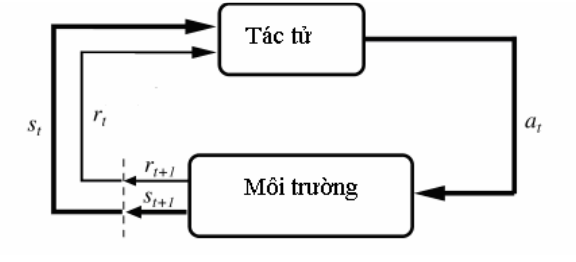
\includegraphics[scale=0.7]{tactumoitruong.png}
    \caption{Mô hình tương tác giữa tác tử và môi trường.}
    \label{fig:tactumoitruong}
\end{figure}

Trong lược đồ trên, tác tử và môi trường tác động lẫn nhau tại mỗi bước trong chuỗi các bước thời gian rời rạc, $t=0,1,2,3,...$. Tại mỗi bước thời gian $t$, tác tử nhận một số biểu diễn về trạng thái của môi trường, $s_t \in S$, với $S$ là tập các trạng thái có thể, và trên đó lựa chọn một hành động $a_t \in A(s_t)$, với $A(s_t)$ là tập các hành động trong trạng thái $s_t$. Mỗi bước thời gian tiếp theo, tác tử nhận một giá trị tăng cường $r_{t+1}\in R$ và tự nó tìm ra một trạng thái mới $S_{t+1}$.
\newline \medskip
Tại mỗi bước tác tử thực hiện ánh xạ từ các trạng thái đến các hành động có thể lựa chọn. Phép ánh xạ này được gọi là chiến lược của tác tử, kí hiệu là $\pi_t$ với $\pi_t(s,a)$ là xác suất thực hiện hành động $a_t=a$ khi $s_t=s$. 

\subsection{Các phần tử của bài toán quyết định Markov}
Dựa vào tác tử và môi trường, chúng ta có thể định nghĩa các phần tử con của một bài toán quyết định Markov: chiến lược (\textit{policy}), hàm phản hồi (\textit{reward function}), hàm giá trị (\textit{value function}), và không bắt buộc, một mô hình về môi trường.
\subsubsection*{Chiến lược}
\textit{Chiến lược} định nghĩa cách thức tác tử học từ hành động tại thời điểm đưa ra. Chiến lược là một ánh xạ từ tập các trạng thái của môi trường đến tập các hành động được thực hiện khi môi trường ở trong các trạng thái đó. Nó tương ứng với tập các luật nhân quả trong lĩnh vực tâm lý học. Trong một số trường hợp, chiến lược có thể là một hàm đơn giản hoặc một bảng tra cứu, trong những trường hợp khác, nó có thể liên quan đến các tính toán mở rộng, ví dụ như một tiến trình tìm kiếm. Chiến lược là nhân của một tác tử với nhận thức rằng một mình nó đủ quyết định hành động.
\newpage
\subsubsection{Hàm phản hồi}
Mục đích của tác tử là cực đại hóa các mục tiêu được tích lũy trong tương lai. Hàm phản hồi $R(t)$ được biểu diễn dưới dạng hàm số đối với các mục tiêu. Trong các bài toán quyết định Markov, hàm phản hồi sử dụng biểu thức dạng tổng. Các nhà nghiên cứu đã tìm ra ba biểu diễn thường được sử dụng của hàm phản hồi:
\begin{itemize}
\item \textit{Trong các bài toán số bước hữu hạn}

Với những bài toán này ta có một số hữu hạn các bước trong tương lai. Sẽ tồn tại một trạng thái kết thúc và một chuỗi các hành động giữa trạng thái đầu tiên và trạng thái kết thúc được gọi là một giai đoạn.
Ta có:
\begin{align*}
R(t)=r_{t}+r_{t+1}+...+r_{t+K-1}
\end{align*}
	Trong đó K là số các bước trước trạng thái kết thúc.
\item \textit{Trong các bài toán số bước vô hạn}\\
	Với những bài toán này ta có chuỗi các hành động là vô hạn. Một hệ số suy giảm $\gamma,0\leq \gamma \leq 1$ được đưa ra và hàm phản hồi được biểu diễn dưới dạng tổng của các giá trị mục tiêu giảm dần:
\begin{align*}
R(t)= \sum_{k=0}^{\infty} \gamma ^{k} r_{t+k}.
\end{align*}
Hệ số $\gamma$ cho phép xác định mức độ ảnh hưởng của những bước chuyển trạng thái tiếp theo đến giá trị phản hồi tại thời điểm đang xét. Giá trị của $\gamma$ cho phép điều chỉnh giai đoạn tác tử lấy các hàm tăng cường. Nếu $\gamma =0$, thì tác tử chỉ xem xét mục tiêu gần nhất, giá trị $\gamma$ càng gần với 1 thì tác tử sẽ quan tâm đến các mục tiêu xa hơn trong tương lai.
Như vậy, thực chất bài toán quyết định Markov trong trường hợp này chính là việc lựa chọn các hành động để làm cực đại biểu thức R:
\begin{align*}
R=r_{0}+\gamma r_{1}+\gamma^{2}r_{2}+... ~\textit{với}~ 0<\gamma <1.
\end{align*}
	Như trong hình vẽ minh họa sau:\\
	
\begin{figure}[ht]
    \centering
    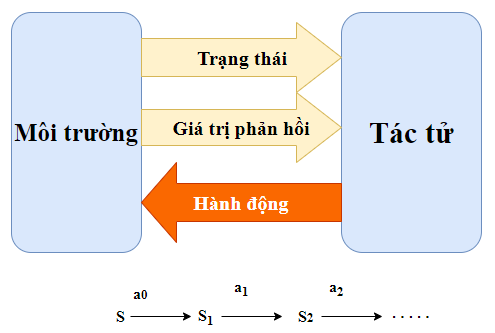
\includegraphics[scale=0.8]{ttmoitruongvohan.png}
    \caption{Mô hình tương tác giữa tác tử và môi trường trong bài toán có số bước vô hạn.}
    \label{fig:tactumoitruong}
\end{figure}
\newpage
\item \textit{Trong các bài toán số bước vô hạn mà hàm phản hồi không hội tụ}

Trường hợp này xảy ra khi $\gamma = 1$. Giá trị trung bình của hàm phản hồi trên một bước thực hiện có thể hội tụ khi số bước tiến tới vô hạn. Trong trường hợp này hàm phản hồi được xác định bằng cách lấy trung bình của các giá trị tăng cường trong tương lai:
\begin{align*}
R(t)=\lim_{n\rightarrow \infty} \frac{1}{n}\sum_{k=0}^{\infty}r_{t+k}.
\end{align*}
\end{itemize}

\subsubsection{Hàm giá trị}
	Trong mọi trạng thái $s_{t}$, một tác tử lựa chọn một hành động dựa theo một chiến lược điều khiển, $ \pi: a_{t}=\pi(s_{t})$. Hàm giá trị tại một trạng thái của hệ thống được tính bằng kỳ vọng toán học của hàm phản hồi theo thời gian. Hàm giá trị là hàm của trạng thái và xác định mức độ thích hợp của chiến lược điều khiển $\pi$ đối với tác tử khi hệ thống đang ở trạng thái $s$. Hàm giá trị của trạng thái $s$ trong chiến lược $\pi$ được tính như sau:
\begin{align*}
V^{\pi}(s)=E_{\pi} \lbrace R_{t}|s_{t}=s\rbrace.
\end{align*}
	Bài toán tối ưu bao gồm việc xác định chiến lược điều khiển $\pi ^{*}$ sao cho hàm giá trị của trạng thái hệ thống đạt cực đại sau một số vô hạn hoặc hữu hạn các bước:
	$$ \pi^{*}= \lbrace \pi_{0}(s_{0}),\pi_{1}(s_{1}),...,\pi_{N-1}(s_{N-1} \rbrace.$$
	Đối với bài toán có số bước vô hạn ta có hàm giá trị trạng thái:
	$$ V^{\pi}(s)=E_{\pi} \lbrace R_{t}=\sum_{k=0}^{\infty}\gamma^{k}r_{t+k+1}|s_{t}=s \rbrace. $$
	Sử dụng các phép biến đổi:
	\begin{align*}
	V^{\pi}(s)&= E_{\pi} \lbrace R_{t}|s_{t}=s \rbrace \\
	&=E_{\pi} \lbrace \sum_{k=0}^{\infty} \gamma^{k} r_{t+k+1}|s_{t}=s \rbrace \\
	&=E_{\pi} \lbrace r_{t+1}+\gamma\sum_{k=0}^{\infty} \gamma^{k}r_{t+k+2}|s_{t}=s \rbrace\\
	&=\sum_{a} \pi(s,a) \sum_{s'} P_{ss'}^{a} [R_{ss'}^{a}+\gamma E_{\pi} \lbrace \sum_{k=0}^{\infty}\gamma^{k}r_{t+k+2}|s_{t+1}=s' \rbrace ]\\
	&=\sum_{a}\pi(s,a) \sum_{s'} P_{ss'}^{a}[R_{ss'}^{a}+\gamma V^{\pi}(s')].
	\end{align*}
	Như vậy, hàm $V^\pi (s)$ có thể được viết lại một cách đệ qui như sau:
$$V^\pi(s)=E_{\pi} {r_{t+1}+\gamma V^\pi (S_{t+1})|S_t=s},$$

hay
\begin{align}\label{1.11}
V^\pi(s)=R(s,a)+\gamma \sum_{s' \in S} P_{ss'}^{a}V^\pi (s').
\end{align}
Với $P_{ss'}^{a}$ là xác suất để chuyển từ trạng thái $s$ sang $s'$ khi áp dụng hành động $a$. Chúng ta có thể tính toán hàm $V^\pi(s)$ ngoại tuyến nếu biết trạng thái bắt đầu và xác suất mọi phép chuyển đổi theo mô hình. Vấn đề đặt ra là sau đó giải quyết hệ thống các phương trình tuyến tính trong công thức \ref{1.11}. Chúng ta biết rằng tồn tại một chiến lược tối ưu, kí hiệu $\pi^*$, được định nghĩa như sau :
\begin{align*}
&V^{\pi^*}(s) \geq V^\pi(s)\\
&\pi^* =argmax_\pi {V^\pi(s)},
\end{align*}
để đơn giản chúng ta viết $V^*=V^{\pi^*}$. Hàm giá trị tối ưu của một trạng thái tương ứng với chiến lược tối ưu là:
$$V^\pi(s)=max_\pi {V^\pi(s)},$$
đây là phương trình tối ưu Bellman (hoặc phương trình của quy hoạch động) ta sẽ nói chi tiết hơn ở phần tiếp theo.\\

Tóm lại $V^\pi$ \textit{là hàm giá trị trạng thái cho chiến lược $\pi$}. Giá trị của trạng thái kết thúc thường bằng $0$. Tương tự, định nghĩa $Q^\pi(s,a)$ là giá trị của việc thực hiện hành động $a$ trong trạng thái $s$ dưới chiến lược điều khiển $\pi$, được tính bằng kỳ vọng toán học của hàm phản hồi bắt đầu từ trạng thái $s$, thực hiện hành động $a$ trong chiến lược $\pi$:
\begin{align*}
.Q^\pi(s,a)=E_\pi \lbrace R_t|s_t=s,a_t=a\rbrace =E_\pi \Big\lbrace \sum_{k=0}^{\infty}\gamma^k r_{t+k+1}|s_t=s,a_t=a \Big \rbrace,
\end{align*}
$Q^\pi$ được gọi là hàm giá trị hành động cho chiến lược $\pi$. Và các hàm giá trị $V^\pi$, $Q^\pi$ có thể được ước lượng từ kinh nghiệm.
\section{Phương trình tối ưu Bellman cho bài toán MDP}

Từ trạng thái $s$, có thể đưa ra nhiều hành động khác nhau và mỗi chiến lược xác định một phân phối xác suất của hành động đó, do đó, sử dụng phương trình tối ưu Bellman để đưa ra quyết định cho bài toán này.\\
Phương trình Bellman cho hàm giá trị trạng thái:
\begin{align*}
V^{\pi}(s)&=R_{\pi}(s)+\gamma \sum_{s'\in S}P_{\pi}(s,s')V^{\pi}(s')\\
&=\sum_{a\in A}\pi(a|s)\left ( R_{a}(s)+\gamma \sum_{s'\in S}P_{\pi}(s,s')V^{\pi}(s') \right ).
\end{align*}
Phương trình Bellman cho hàm giá trị hành động:
\begin{align*}
Q^{\pi}(s,a)=R_{a}(s)+\gamma \sum_{s'\in S} P_{a}(s,s')\sum_{a' \in A}\pi(a'|s')Q^{\pi}(s',a').
\end{align*}
\begin{dn} \rm
Hàm giá trị trạng thái tối ưu $V^{*}(s)$ là hàm trả về trạng thái tối ưu trên tất cả các chiến lược:
\begin{align*}
V^{*}(s)~=~\displaystyle\max_{\pi} V^{\pi}(s).
\end{align*}
\end{dn}
\begin{dn} \rm
Hàm giá trị hành động tối ưu $Q^{*}(s,a)$ là hàm trả về các hành động tối ưu trên tất cả các chiến lược:
\begin{align*}
Q^{*}(s,a)~=~\displaystyle\max_{\pi} Q^{\pi}(s,a).
\end{align*}
\end{dn}

\begin{dn}\rm 
(Chiến lược tối ưu) $\pi$ được gọi là chiến lược tối ưu nếu $V^{\pi}(s) \geq V^{\pi '}(s), \forall s.$\\
Xác định một chiến lược tối ưu: Một chiến lược tối ưu có thể được xác định bằng cách tìm hàm cực đại $Q^{*}(s,a)$:
\begin{align}
\pi^{*}(a|s)=\begin{cases}
1 & \text{ nếu } a=argmax_{a\in A}~Q^{*}(s,a) \\ 
0 & \text{ ngược lại } 
\end{cases}
\end{align}
Phương trình tối ưu Bellman cho $V^{*}(s)$:
\begin{align}
V^{*}(s)= \displaystyle\max_{a}~ R_{a}(s)+\gamma \sum_{s'\in S}P_{a}(s,s')V^{*}(s').
\end{align}
Phương trình tối ưu Bellman cho $Q^{*}(a,s)$:
\begin{align}
Q^{*}(s,a)=R_{a}(s)+\gamma \sum_{s'\in S}P_{a}(s,s') \displaystyle\max_{a'}~Q^{*}(s',a').
\end{align}
Phương trình tối ưu Bellman là một phương trình phi tuyến có thể giải bằng một số phương pháp: lặp giá trị và lặp chính sách.
\end{dn}